% NOTE : COMMENT ON TRACE LE DEPLACREMENT -> MOYENNE AU NOEUDS A PRECISER DANS LA LEGENDE DE LA FIGURE
% NOTE : LE CODE, CE QU'ON UTILISE, MFRONT MGIS -> IMPLEMENTATION PORTEE DANS CAST3M -> IMPLEMENTATION PLUGGABLE DANS AUTRE CHOSE -> 
% NOTE : ON PARLE PAS DES TEMPS DE CALCULS DANS LA SUITE parce que c du python, on montr que les 2 schémas d'intégration convergecne de manière qudartique, localement et globalement
% POUR ETRE COHERENT EN CONDENSATION, IL FAUT ACCLERER LES FACES +  LES CELLULES. POUR NOUS C QUE LES FACES


% ---------------------------------------------------------
% ---- SECTION
% ---------------------------------------------------------
\section{Numerical examples in the axisymmetric modelling hypothesis}
\label{sec_numerical_examples}

In this section, the proposed axi-symmetric HHO method is evaluated on
classical test cases taken from the literature to emphasize robustness
to volumetric locking.
The reader can refer to \ref{sec_appendix_axi} regarding technical aspects on the formulation of the proposed HHO method for the axisymmetric modelling hypothesis. 
Both the small and large strains
frameworks are considered, for elasto-plastic behaviors. The notation
HHO($k,l$) relates to the HHO element of order $k$ on faces, and order $l$ in the
cell.

The tests presented in this section have been performed using an
\texttt{python} implementation freely available on github: \url{https://github.com/davidsiedel/h2o_paper}.
The results of this implementations were thoroughly compared to the
results obtained with the reference implementation provided by the
\texttt{Disk++} solver \cite{cicuttin_implementation_2018} in the cartesian framework.

% ---------------------------------------------------------
% PARAGRAPH
% ---------------------------------------------------------
\paragraph{Stabilization parameter}

To ensure coercivity of the HHO method, the so-called \textit{stabilization} parameter
$\beta$, that relates to the Young modulus of the elastic interface introduced in Section \ref{sec_hdg_element_equilibrium}, needs be chosen according to the material under study. In \cite{di_pietro_hybrid_2015}, a value of
order $2 \mu$ is advocated, where $\mu$ denotes the shear modulus of the
material. This value is used for all test cases in the present section.

% ---------------------------------------------------------
% -- SUBSECTION
% ---------------------------------------------------------
\subsection{The free dilatation test}
\label{sec_satoh_test}

The first test case of the following benchmark aims at displaying the
robustness of the HHO method for coupled mechanical-thermal problems.

% ---------------------------------------------------------
% PARAGRAPH
% ---------------------------------------------------------
\paragraph{Specimen and loading}

For this test case, the unit box is fixed on both the right and
bottom boundaries in their respective normal directions, and a quadratic
thermal load depending on the $r$-coordinate is imposed in the solid
(see Figure \ref{fig_satoh_setting}). The mesh is composed of 400
quadrangles. The thermal loading is given by:
%
%
%
\begin{equation}
    T(r,z) = 4 (T_{max} - T_{min}) \, r \, (1 - r) + T_{min}
\end{equation}
%
%
%
with temperature values $T_{max} = 2000$ K and $T_{min} = 293.15$ K.

\begin{figure}[H]
    \centering
    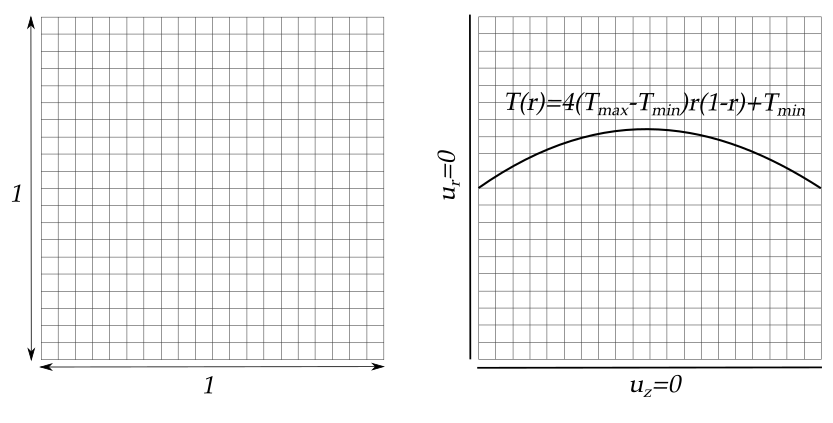
\includegraphics[width=10.cm]{../chapter_002_hho_mechanics/figures/satoh_setting.png}
    \caption{Geometry, displacement boundary conditions and temperature loading for the free dilatation test case}
    \label{fig_satoh_setting}
\end{figure}

% ---------------------------------------------------------
% PARAGRAPH
% ---------------------------------------------------------
\paragraph{Material behaviour}

A linear thermo-elastic energy potential is considered with a Young's
modulus $E$ equal to $150$ GPa. The material is quasi-incompressible
with a Poisson's ratio $\nu$ equal to $0.499$. The dilatation parameter
is taken as $\alpha = 1e^{-6}$ K$^{-1}$.

% ---------------------------------------------------------
% PARAGRAPH
% ---------------------------------------------------------
\paragraph{Volumetric locking and polynomial approximation for the strain and temperature fields}

A sign of volumetric locking is the presence of strong oscillations in the trace of the Cauchy stress (or, equivalently, the hydrostatic pressure) within elements.
Using Lagrange finite elements of order respectively $1, 2$, the
strain approximation is of order $0, 1$, whereas the thermal
strain adopted in this example is of order $2$, which results in strong signs of volumetric locking. For Lagrange
elements to accurately model the hydrostatic pressure, one needs to choose a polynomial approximation of the temperature field that is one order lower than that of the
displacement field. This feature is of major importance for mixed
elements, where quadratic displacement elements needs be employed together with linear ones for the pressure/swelling field.

\begin{figure}[H]
    \centering
    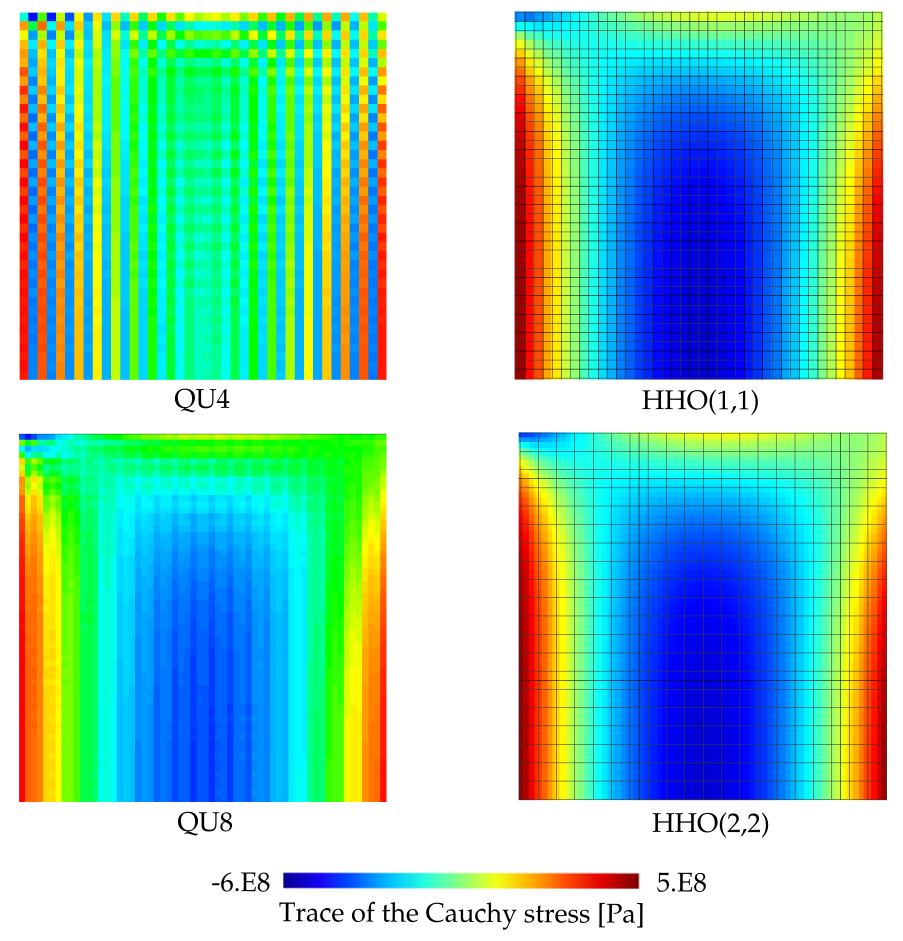
\includegraphics[width=10.cm]{../chapter_002_hho_mechanics/figures/satoh_calc.png}
    \caption{Map fo the Trace of the Cauchy stress at quadrature points for the Free dilatation test case at the last time step}
    \label{fig_satoh_calc}
\end{figure}

% ---------------------------------------------------------
% PARAGRAPH
% ---------------------------------------------------------
\paragraph{Comparison of FE and HHO methods}

In Figure \ref{fig_satoh_calc}, one can observe that the pressure map is completely smooth for HHO computations, even for a quadratic temperature field acting on a linear gradient using HHO(1,1). As expected, the results display mild signs of volumetric locking for the quadratic finite element
approximation, and strong oscillations are noted for the linear finite element solution.

% ---------------------------------------------------------
% -- SUBSECTION
% ---------------------------------------------------------
\subsection{Perfect plastic swelling sphere}
\label{sec_swelling_sphere}

% ---------------------------------------------------------
% PARAGRAPH
% ---------------------------------------------------------
\paragraph{Specimen and loading}

This benchmark consists in a quasi-incompressible sphere under uniform internal loading (see Figure \ref{fig_sphereall}).
This test case has an analytical solution and the state of the specimen is known when the plastic region has reached the external border of the sphere.
The sphere has an inner radius $r_{int} = 0.8$ mm and an outer
radius $r_{ext} = 1$ mm. An internal radial displacement $u$ is imposed.
The simulation is performed until the limit load corresponding to an internal displacement of $0.2$ mm is reached.

% ---------------------------------------------------------
% PARAGRAPH
% ---------------------------------------------------------
\paragraph{Material behaviour}

An isotropic hardening energy potential $\mecPotential{}_{\bodyLag{}}^p$ is chosen for the description of the plastic evolution of the material such that

\begin{equation}
    \mecPotential{}_{\bodyLag{}}^p(p)
    =
    \sigma_0 p + \frac{1}{2} H p^2 + (\sigma_{\infty} - \sigma_0)(p - \frac{1 - e^{-\delta p}}{\delta})
\end{equation}
%
%
%
where the parameter $p$ denotes the equivalent plastic strain and a Von Mises yields function $f$ describes the flow rule
%
%
%
\begin{equation}
    f = \sqrt{\frac{3}{2}} \rVert \text{dev} (\tensorii{\sigma}) \lVert - p
\end{equation}
%
%
%
Moreover, the small strain hypothesis is assumed, and
perfect plasticity is considered for this test case. The saturation parameter $\delta$ and the hardening parameter $H$ are taken to $0$, the yield stresses are such that $\sigma_0 = \sigma_{\infty} = 6$ MPa, and the elastic potential parameters are the Young modulus $E = 28.85$ MPa and the Poisson ratio $\nu = 0.499$, such that the material is quasi-incompressible.

\begin{figure}[H]
    \centering
    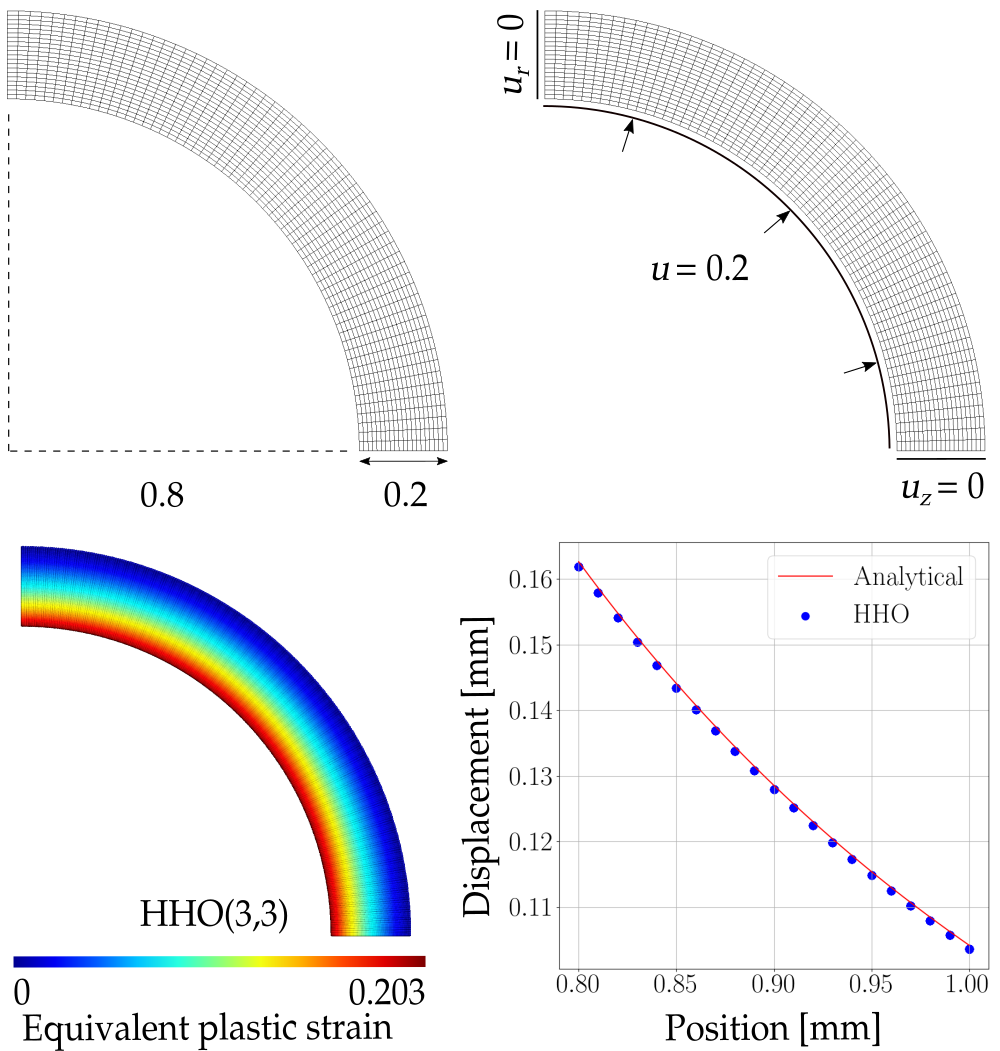
\includegraphics[width=12.cm]{../chapter_002_hho_mechanics/figures/sphere_mesh.png}
    \caption{the swelling sphere test case. Geometry, loadings, final displacement along the radius of the sphere, and final equivalent plastic strain map at quadrature points}
    \label{fig_sphereall}
\end{figure}

% ---------------------------------------------------------
% PARAGRAPH
% ---------------------------------------------------------
\paragraph{Displacement along the radius}

Since an analytical solution is known for this test case, it is compared to the proposed HHO method numerical results. The displacement of the section of the sphere at cell nodes
is plotted in Figure \ref{fig_sphereall}, along with the analytical one, and it is noticed that the obtained results are in agreement with the analytical ones.
Figure \ref{fig_sphereall} mentions the label HHO without specifying approximation orders for all computations deliver the same result.

% ---------------------------------------------------------
% PARAGRAPH
% ---------------------------------------------------------
\paragraph{Trace of the Cauchy stress}

As for the displacement, the analytical solution for the trace of the Cauchy stress tensor is compared to the one computed using the proposed HHO method for three approximation orders.
Numerical results at quadrature points fit the analytical curve, and display no sign of volumetric locking. The computed solution is however less smooth
at the borders of the specimen for higher orders, a phenomenon that was pointed out in \cite{abbas_hybrid_2019-1} for the three dimensional case, and attributed to the fact that planar faces are considered.

\begin{figure}[H]
    \centering
    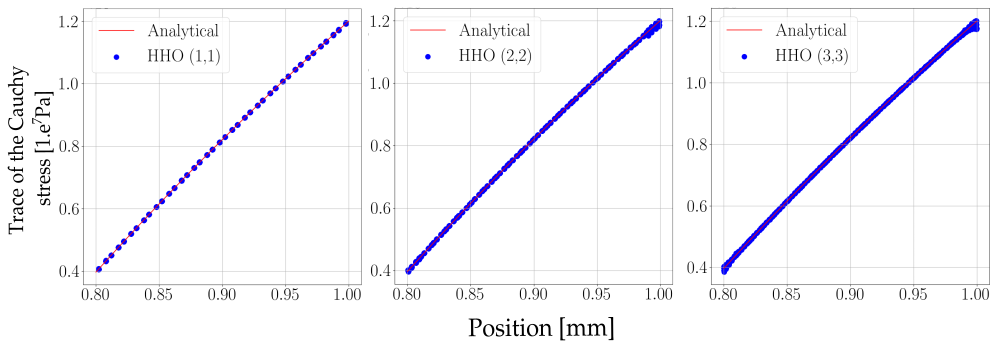
\includegraphics[width=15.cm]{../chapter_002_hho_mechanics/figures/sphere_pressures.png}
    \caption{trace of the Cauchy stress tensor along the radius of the sphere at quadrature points}
    \label{fig_sphere_pressure}
\end{figure}

% ---------------------------------------------------------
% -- SUBSECTION
% ---------------------------------------------------------
\subsection{Necking of a notched bar}

% ---------------------------------------------------------
% PARAGRAPH
% ---------------------------------------------------------
\paragraph{Specimen and loading}

The last application consists of a notched bar that is subjected to uniaxial
extension.
The bar has a length of $30$ mm, a top section of radius $5$ mm and a bottom section of radius $3$ mm.
A vertical
displacement $u_z = 0.8$ mm is imposed at the top, as shown in Figure \ref{fig_ssnaallmesh}.
For symmetry reasons, only one-quarter of the
bar is discretized.

% ---------------------------------------------------------
% PARAGRAPH
% ---------------------------------------------------------
\paragraph{Behaviour law}

The same behavior law as that in \ref{sec_swelling_sphere} is considered for the present test case. 
However, the finite strain hypothesis is chosen, based on a logarithmic decomposition of the stress \cite{miehe_anisotropic_2002}.

% ---------------------------------------------------------
% PARAGRAPH
% ---------------------------------------------------------
\paragraph{Material parameters}

Materials parameters are taken as
$\sigma_0 = 450$ MPa, $\sigma_{\infty} = 715$ MPa with a saturation parameter $\delta = 16.93$. The Young modulus is $E = 206.9$ GPa, and the Poisson ratio is $\nu = 0.29$.

% ---------------------------------------------------------
% PARAGRAPH
% ---------------------------------------------------------
\paragraph{Load deflection curve}

The load-displacement curve is plotted
in Figure \ref{fig_ssnaallmesh}, and gives similar results to that obtained with quadratic reduced integration elements.

% ---------------------------------------------------------
% PARAGRAPH
% ---------------------------------------------------------
\paragraph{Equivalent plastic strain}

Moreover, the equivalent
plastic strain $p$ at quadrature points and at the final load is plotted Figure \ref{fig_ssnaallplastic}.
It has been observed that the equivalent plastic strain might suffer some oscillations at a certain limit load with UPG methods.
One notices through the present example, that the proposed HHO method displays no oscillations of the equivalent plastic strain.

\begin{figure}[H]
    \centering
    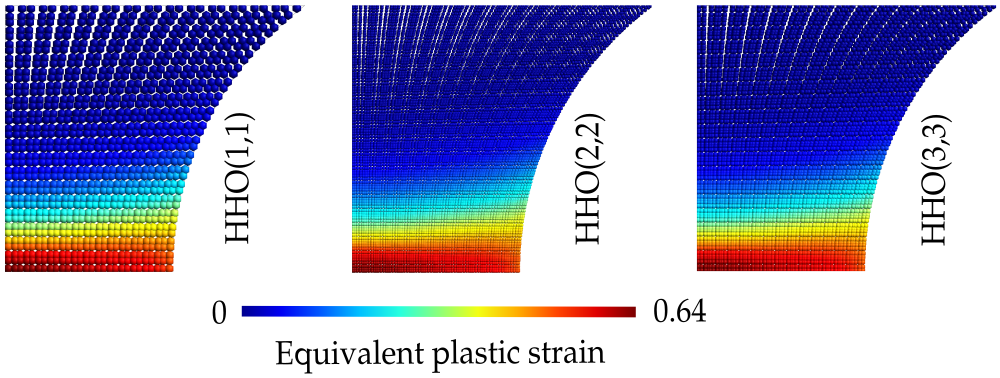
\includegraphics[width=12.cm]{../chapter_002_hho_mechanics/figures/ssna_plastic.png}
    \caption{
        final equivalent plastic strain map at quadrature points in the notch region
    }
    \label{fig_ssnaallplastic}
\end{figure}

% ---------------------------------------------------------
% PARAGRAPH
% ---------------------------------------------------------
\paragraph{Hydrostatic pressure}

The hyrostatic pressure map at quadrature points and at the final load is shown Figure \ref{fig_ssnaallmesh} for three HHO element orders (respectively $1, 2$ and $3$).
As for the swelling sphere test case, one notices that the hydrostatic pressure map is
fairly smooth over the whole structure at all approximation orders, even at the bottom left corner where plasticity is confined.

\begin{figure}[H]
    \centering
    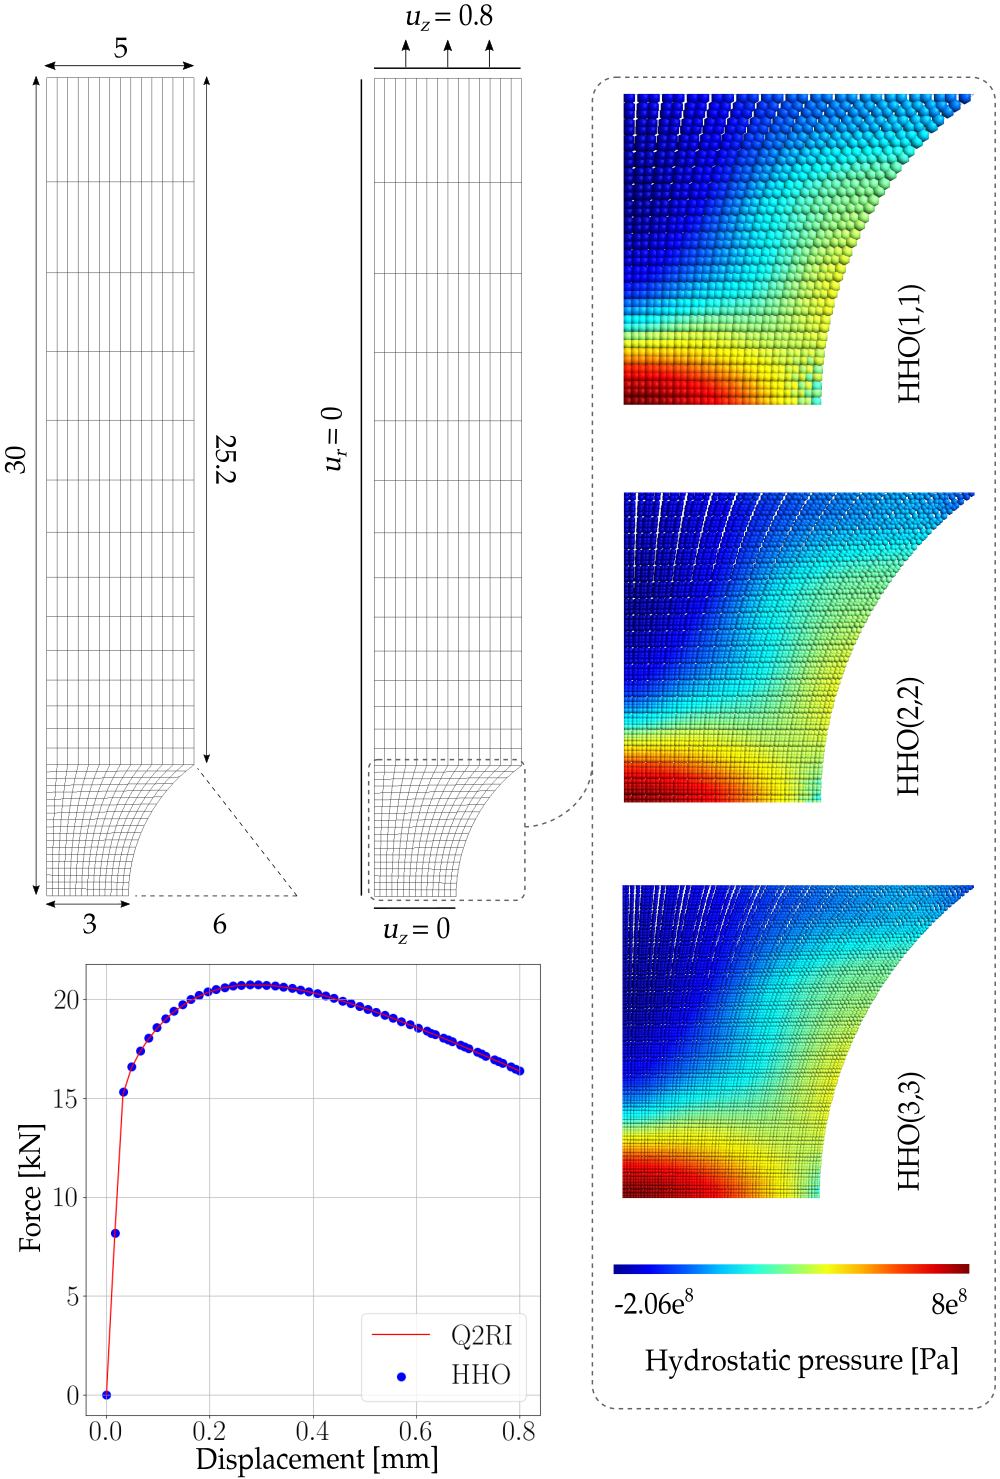
\includegraphics[width=12.cm]{../chapter_002_hho_mechanics/figures/ssna_mesh.png}
    \caption{
        the notched specimen test case. Geometry, loadings, load deflection curve, and final hydrostatic pressure map at quadrature points in the notch region
    }
    \label{fig_ssnaallmesh}
\end{figure}

% ---------------------------------------------------------
% ---- SUBSECTION
% ---------------------------------------------------------
\subsection{Comparison of cell unknowns elimination schemes}
\label{sec_num_example_part_2}

In this section, both elimination strategies
introduced in Section \ref{sec_cell_unknowns_elimination} are evaluated. In particular, four different variants of the usual
Newton algorithm
are studied, namely :
% \begin{itemize}
%     \item (R) the Static condensation scheme using a consistent Jacobian operator
%     \item (M1) the Cell equilibrium scheme using a consistent Jacobian operator
%     \item (M2) the Static condensation scheme using an elastic Jacobian operator
%     \item (M3) the Cell equilibrium scheme using an elastic Jacobian operator
%     \item (M4) the Static condensation scheme using an elastic Jacobian operator and coupled with an Anderson acceleration algorithm, that acts on both cell and faces unknowns at the global level
%     \item (M5) the Cell equilibrium scheme using an elastic Jacobian operator coupled with an Anderson acceleration algorithm on faces unknowns only
% \end{itemize}
(Sc) a Static condensation scheme using a consistent Jacobian operator,
(Cc) a Cell equilibrium scheme using a consistent Jacobian operator,
(Se) a Static condensation scheme using an elastic Jacobian operator,
(Ce) a Cell equilibrium scheme using an elastic Jacobian operator,
(Sa) a Static condensation scheme using an elastic Jacobian operator and coupled with an Anderson acceleration algorithm, that acts on both cell and faces unknowns at the global level,
(Ca) a Cell equilibrium scheme using an elastic Jacobian operator coupled with an Anderson acceleration algorithm on faces unknowns only.

The last two test cases that showcase non-linear behaviours are considered for the evaluation of all these variants. The static condensation resolution scheme that uses a consistent stiffness matrix is taken for reference, since it is the
one used in the literature \cite{abbas_hybrid_2019,abbas_hybrid_2018}.
The estimation of the Anderson acceleration is performed every iteration and is based on the last three residual and unknown vectors.

\paragraph{Number of iterations per time step}

The number of iterations per time step for each variant
is displayed in Figure \ref{fig_acceleration_res_0} for both the swelling sphere test case
and the notched rod one.
At each time steps, the number of iteration is normalized by the number of iterations obtained with the
Static condensation variant (Sc).
As expected, the number of iteration per time step is similar for Cell resolution scheme based variants and Static condensation ones, for all polynomial orders and all alternatives listed above.

\begin{figure}[H]
    \centering
    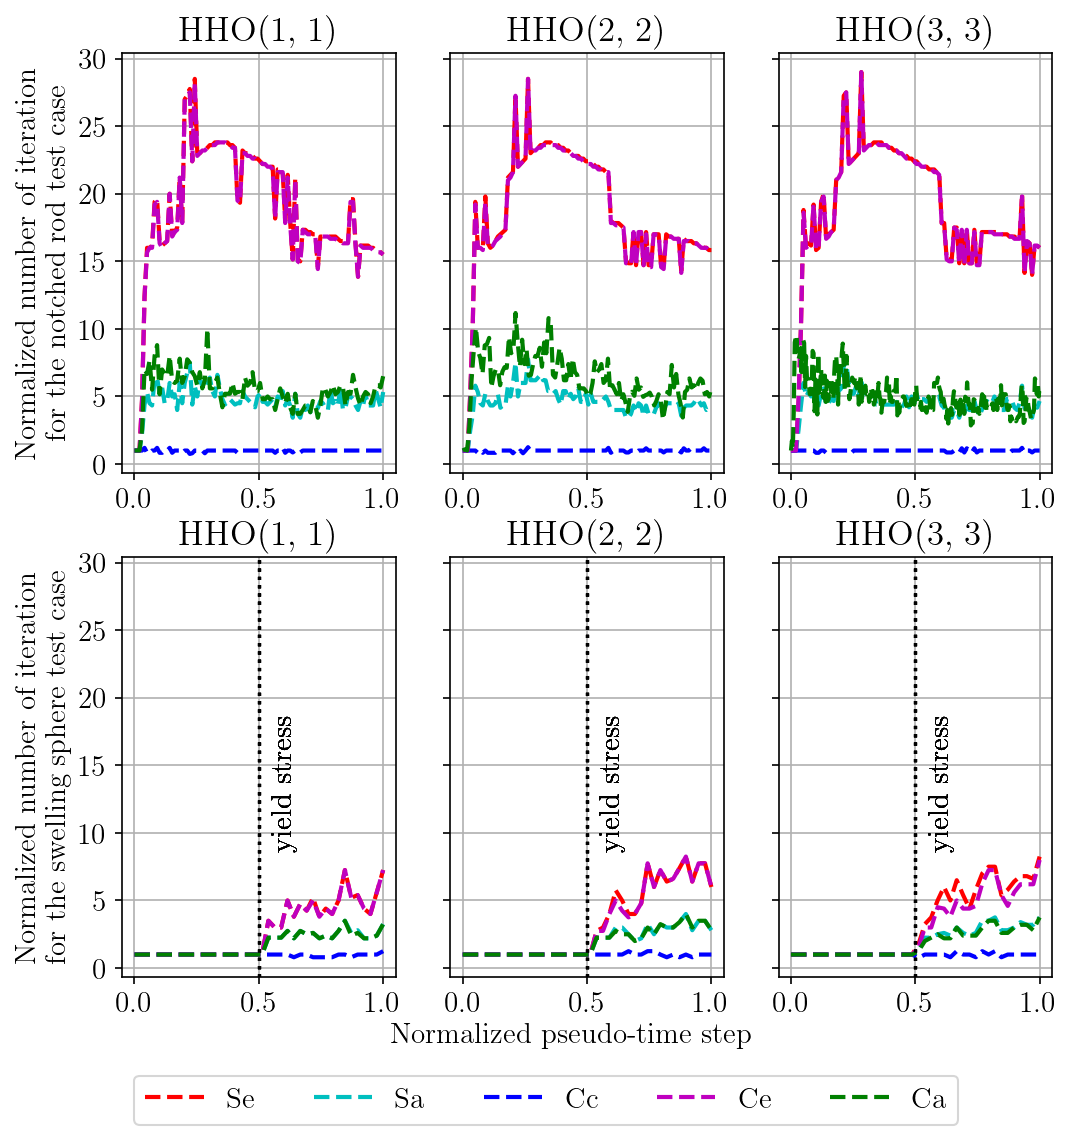
\includegraphics[width=12.cm]{../chapter_002_hho_mechanics/figures/plot_global_iterations__4_ordn.png}
    \caption{Normalized number of iterations per time step for non-linear test cases and all resolution schemes variants}
    \label{fig_acceleration_res_0}
\end{figure}

\paragraph{Accelereated variants comparison}

The key argument in using the
Cell equilibrium scheme with an acceleration step is that 
only faces unknowns are accelerated.
Using the static condensation scheme demands to accelerate both cell and faces unknowns simultaneously.
However, using the Cell equilibrium scheme, the update of the cell unknown after a sole face acceleration step is performed at the cell level.
From a mechanical standpoint, faces unknowns are perturbed, and solving non-linear equation \eqref{eq_cell_equilibrium_1} by a local Newton algorithm as depicted in Section \ref{sec_cell_equilibrium_scheme} allows to retrieve the cell unknown increment verifying the equilibrium of the element.

\paragraph{Memory footprint}

In addition, local matrices used for the decondensation step in the Static condensation scheme are not kept from one iteration
to another using the Cell equilibrium scheme, hence drastically reducing the total memory footprint of the computation.
The number of scalar values to be stored between each iteration for a cell $\cell$ and for each variant is given in Table \ref{table_memory_footprint}, where $d$ is the number of components of the unknown field,
$M^l_T$ is the size of a scalar cell polynomial unknown, $M^l_T$ is that of a face, $N_{\dCell}$ is the number of faces for the cell $T$, and
$N_{it}$ denotes the number of residual and associated unknowns to be stored by the Anderson acceleration algorithm.

\begin{table}[H]
    \centering
    \begin{tabular}{||c c||} 
        \hline
        Resolution Method & Memory footprint
        \\
        [0.5ex] 
        \hline\hline
        (Sc), (Se) & $d \, M^l_T (M^k_{\dCell} \, N_{\dCell} + M^l_T)$
        \\ \hline
        (Cc), (Ce) & 0
        \\ \hline
        (Sa) & $d \, M^l_T (M^k_{\dCell} \, N_{\dCell} + M^l_T) + d \, 2 \, N_{it} (M^k_{\dCell} \, N_{\dCell} + M^l_T) $
        \\ \hline
        (Ca) & $d \, 2 \, N_{it} (M^k_{\dCell} \, N_{\dCell})$
        \\ \hline
    \end{tabular}
    \caption{Memory footprint for each alternative and for an element}
    \label{table_memory_footprint}
\end{table}

The number of scalar values that need be stored from one iteration to another for a single quandrangular element, depending on the discretization, and on the chosen acceleration scheme (\textit{i.e.} on the number of resiudal and unknown vectors to store)
is given in Figure \ref{fig_acceleration_res_memory} for different acceleration strategies, cell and faces polynomial orders.

\begin{figure}[H]
    \centering
    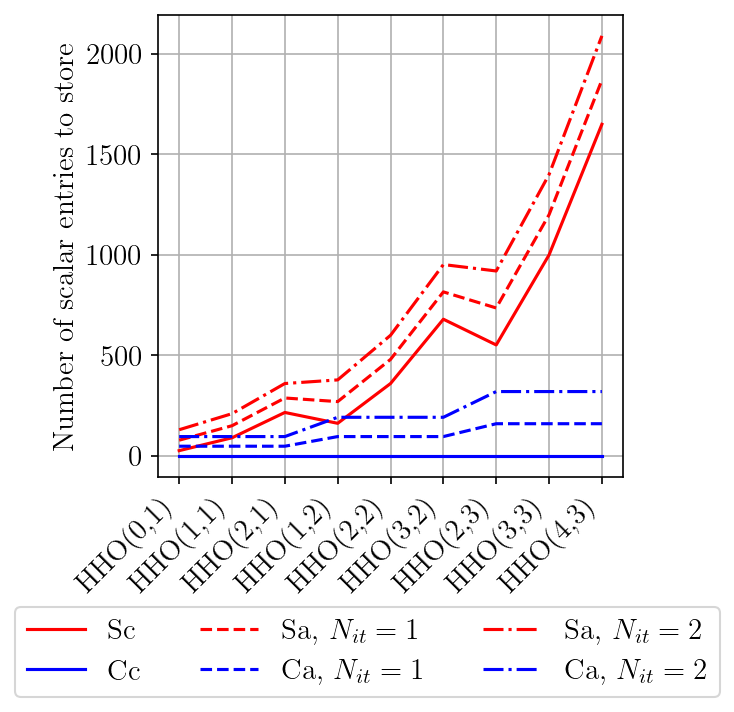
\includegraphics[width=8.cm]{../chapter_002_hho_mechanics/figures/plot_memory.png}
    \caption{Number of scalar entries to store from one iteration to another for different polynomial orders and resolution schemes variants}
    \label{fig_acceleration_res_memory}
\end{figure}

\paragraph{Local iterations}

The price for alleviating the memory footprint of the Static condensation scheme
is paid by systematic calls to the local Newton algorithm.
As a consequence, one also notices an increasing number of calls to the behaviour law.
The mean number of local cell iterations per time time step is given in Figure \ref{fig_acceleration_res_1} for both test cases. The high number of cell iterations for the swelling sphere test case is
due to the fact that the plastic front involves a linearly increasing number of cells submitted to a perfect plastic beahviour.
Considering \textit{e.g.} a linear hardening behaviour law leads to a stabilized number of cell iterations once the whole domain is plastic.

\begin{figure}[H]
    \centering
    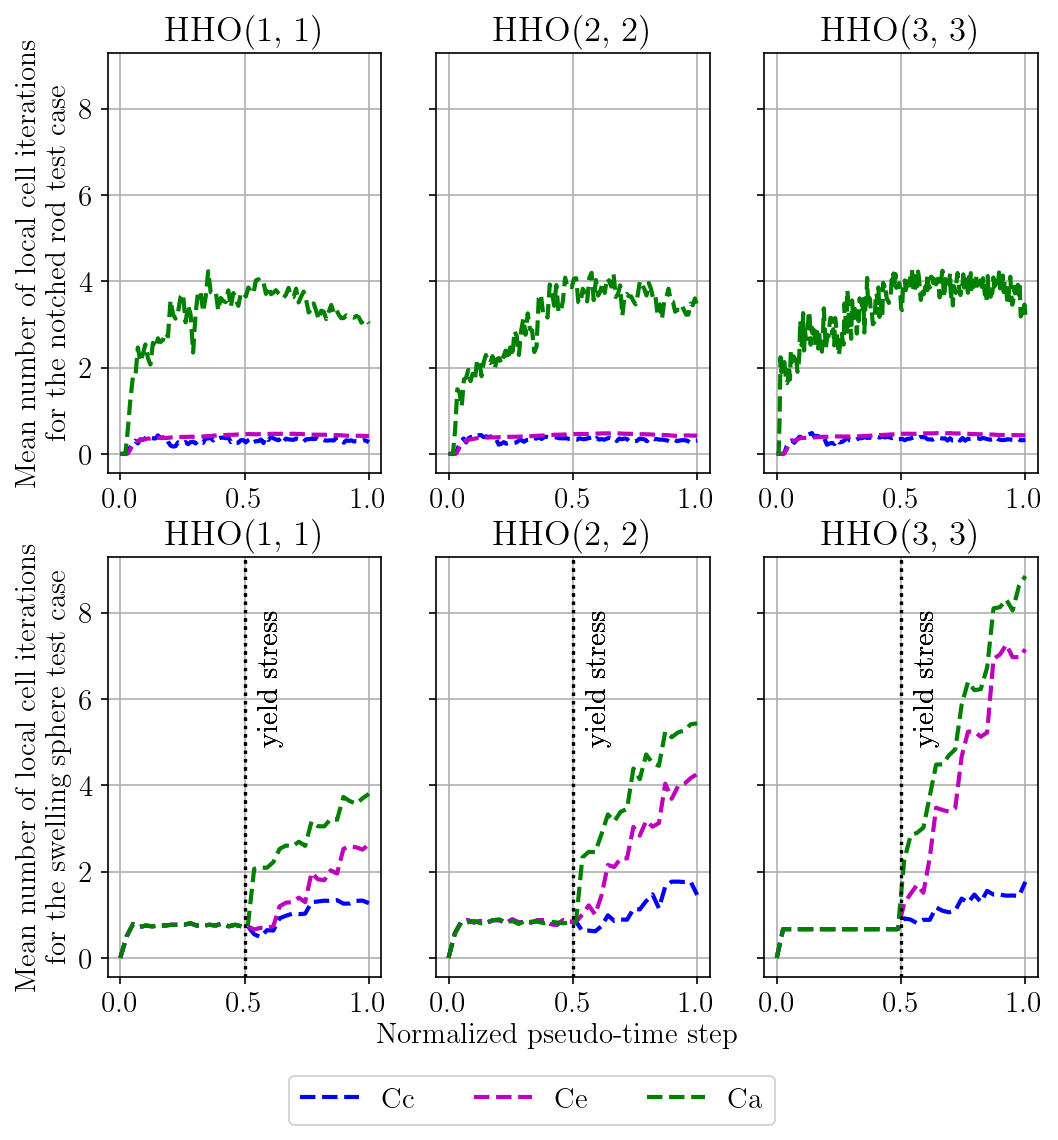
\includegraphics[width=12.cm]{../chapter_002_hho_mechanics/figures/plot_cell_iterations__4_cell_iters.png}
    \caption{Normalized number of cell iterations per time step for non-linear test cases and Cell equilibrium based resolution schemes variants}
    \label{fig_acceleration_res_1}
\end{figure}

\paragraph{Local system}

The local system to solve with each cell scales with the size of a single cell unknown. An overview of the values taken using a monomial shape function can be found in \ref{sec_appendix_implementation}. These local resolution procedures consist in solving dense systems and are completely
parallelizable.

% \subsubsection{Quadratic and accelerated schemes}

% Both the Cell equilibrium and Static condensation resolution schemes are compared in terms of number of global iterations, using either
% a consistent stiffness matrix, an elastic operator, and an elastic operator coupled with an Anderson acceleration
% algorithm.
% The static condensation resolution scheme that uses a consistent stiffness matrix is taken for reference, since it is the
% one used in the literature \cite{abbas_hybrid_2019,abbas_hybrid_2018}.

% \paragraph{Resolution schemes using a consitent stiffness matrix}

% The number of iterations per time step for the Cell equilibrium algorithm using a consistent tangent operator
% is showcased by the dashed blue line in Figure \ref{fig_acceleration_res_0} for the swelling sphere test case,
% and in Figure \ref{fig_acceleration_res_1} for the notched rod one.
% Results are normalized by those obtained with the Static condensation algorithm.
% As expected, the number of iteration per time is roughly the same between the Cell resolution scheme
% and the Static condensation one, for all polynomial orders.

% \paragraph{Resolution schemes using an elastic stiffness matrix}

% Keeping the first elastic stiffness matrix for the whole computation showcases assets that are discussed in Section \ref{sec_cell_unknowns_elimination}. In this section, four resolution methods based on the elastic stiffness matrix are studied :
% \begin{itemize}
%     \item (M1) the Static condensation scheme
%     \item (M2) the Cell equilibrium scheme
%     \item (M3) the Static condensation scheme, coupled with an Anderson acceleration algorithm, that acts on both cell and faces unknowns at the global level
%     \item (M4) the Cell equilibrium scheme, coupled with an Anderson acceleration algorithm on faces unknowns only
% \end{itemize}
% %
% %
% %
% The number of iterations 
% (M1) the Static condensation scheme, (M2) the Cell equilibrium scheme, (M3) the Static condensation scheme, coupled with
% an Anderson acceleration algorithm, that acts on both cell and faces unknowns at the global level and (M4) the Cell
% equilibrium scheme, coupled with an Anderson acceleration algorithm for faces unknowns only.

% \paragraph{}

% Figure \ref{fig_acceleration_res_0} gives the number of iterations needed to achieve convergence
% at the skeletal level, with respect to the current pseudo-time step. The computation is performed
% in $40$ uniform steps from an initial steady state up to the limit radial load of $0.2$ mm (see \ref{sec_swelling_sphere}).
% For this experiment, three variants of both cell elimination schemes are considered :
% \begin{itemize}
%     \item A first scheme S1 consists in using a consistent tangent operator for the computation of the stiffness matrix
%     \item A second scheme S2 consists in using an elastic tangent operator for the computation of the stiffness matrix
%     \item A last scheme consists in us
% \end{itemize}